\documentclass[DaoFP]{subfiles}
\begin{document}
 \setcounter{chapter}{16}

 \chapter{Ends and Coends(极限与余极限)}

 \section{Profunctors(泛函)}

 在范畴论的高度抽象中,我们会遇到一些模式,这些模式离其起源如此遥远,以至于我们难以将其具象化。更为抽象的模式通常与其具体实例的相似度更低,这使得我们理解起来更加困难。

 从$a$到$b$的箭头(arrow)相对容易理解。我们对它有一个非常熟悉的模型:一个函数,它消耗$a$的元素并生成$b$的元素。态射集(hom-set)是一组这样的箭头的集合。

 函子(functor)是范畴之间的箭头。它消耗来自一个范畴的对象和箭头,并生成另一个范畴中的对象和箭头。我们可以将其视为一种使用源范畴提供的材料来构建这些对象(和箭头)的配方。尤其是,我们通常将自函子(endofunctor)视为构建材料的容器。

 泛函(profunctor)将一对对象$\langle a, b \rangle$映射到一个集合$P\langle a, b \rangle$,并将一对箭头
 \[ \langle f \colon s \to a, g \colon b \to t \rangle \]
 映射到一个函数:
 \[ P\langle f, g \rangle \colon P\langle a, b \rangle \to P\langle s, t \rangle \]

 泛函是结合了许多其他抽象元素的抽象。因为它是一个从$ \mathcal{C}^{op} \times  \mathcal{C}$到$\mathbf{Set}$的函子,我们可以将其视为从一对对象中构造一个集合,并从一对箭头(其中一个箭头的方向相反)中构造一个函数。然而,这并不有助于我们进行想象。

 幸运的是,我们有一个关于泛函的良好模型:同态函子(hom-functor)。在变动对象时,两者之间的箭头集表现得像一个泛函。并且明显的是,改变源对象和目标对象的同态集(hom-set)之间存在区别。

 因此,我们可以将任意泛函视为同态函子的泛化。泛函在已有的同态集基础上,为对象之间提供了额外的桥梁。

 然而,泛函$ \mathcal{C}(a, b)$的元素与集合$P\langle a, b \rangle$的元素之间有一个很大的区别。前者的元素是箭头,而箭头可以组合(compose)。对于泛函如何组合,并没有一目了然的方法。

 当然,可以认为泛函通过提升箭头(lifting of arrows)来泛化组合——不过不是在泛函之间,而是在同态集与泛函之间。例如,我们可以用箭头$f \colon s \to a$来“预组合”$P \langle a, b \rangle$,以得到$P \langle s, b \rangle$:
 \[ P\langle f, id_b \rangle \colon P \langle a, b \rangle \to P \langle s, b \rangle \]
 类似地,我们可以用$g \colon b \to t$“后组合”它:
 \[ P \langle id_a, g \rangle \colon P \langle a, b \rangle \to P \langle a, t \rangle \]
 这种异质的组合方式,接受由一个箭头和一个泛函元素组成的可组合对,并生成一个泛函的元素。

 泛函可以通过提升一对箭头在两侧进行扩展:

 \[
  \begin{tikzcd}
   & s
   \arrow[r, bend left, dashed, blue, "f"]
   & a
   \arrow[r, bend right, "P"]
   & b
   \arrow[r, bend left, dashed, blue, "g"]
   &  t
  \end{tikzcd}
 \]

 \subsection{Collages(拼接)}

 没有理由将泛函限制在单一范畴上。我们可以轻松定义一个在两个范畴之间的泛函,例如$ P \colon \mathcal{C}^{op} \times  \mathcal{D} \to \mathbf{Set}$。这样的泛函可以通过生成从$\mathcal{C}$中的对象到$\mathcal{D}$中的对象的同态集(hom-set)来将两个范畴连接在一起。

 两个范畴$\mathcal{C}$和$\mathcal{D}$的拼接(collage)是一个范畴,其对象是来自两个范畴的对象(不相交的并集)。对于两个对象$x$和$y$之间的同态集,要么是$\mathcal{C}$中的同态集(如果两个对象都在$\mathcal{C}$中);要么是$\mathcal{D}$中的同态集(如果两个对象都在$\mathcal{D}$中);要么是集合$P \langle x, y\rangle$(如果$x$在$\mathcal{C}$中,$y$在$\mathcal{D}$中)。否则,同态集是空的。

 态射的组合是通常的组合方式,除非其中一个态射是$P \langle x, y \rangle$的元素。这种情况下,我们需要提升我们尝试进行前组合或后组合的态射。

 很容易看出,拼接确实是一个范畴。新的态射跨越了拼接的两边,有时被称为异态射(heteromorphisms)。它们只能从$\mathcal{C}$到$\mathcal{D}$,而不能反向进行。

 从这个角度看,一个从$ \mathcal{C}^{op} \times  \mathcal{C}$到$\mathbf{Set}$的泛函应该真正被称为一个\emph{内}泛函(endo-profunctor)。它定义了$\mathcal{C}$与其自身的拼接。

 \begin{exercise}
  证明从两个范畴的拼接到一个有两个对象和一个箭头(以及两个恒等箭头)的“步行箭头”范畴(walking arrow category)之间存在一个函子。
 \end{exercise}

 \begin{exercise}
  证明,如果从$\mathcal{C}$到步行箭头范畴存在一个函子,那么$\mathcal{C}$可以分解成两个范畴的拼接。
 \end{exercise}

 \subsection{Profunctors as relations(作为关系的泛函)}

 在微观层面上,泛函看起来像一个同态函子,并且集合$P \langle a, b \rangle$的元素看起来像个别箭头。但是,当我们放大观察时,可以将泛函视为对象之间的关系。这些关系不是普通的关系;它们是\emph{证明相关关系}(proof-relevant relations)。

 为了更好地理解这一概念,让我们考虑一个普通的函子$F \colon \mathcal{C} \to \mathbf{Set}$(换句话说,一个余预层(co-presheaf))。可以将其解释为,它定义了$\mathcal{C}$对象的一个\emph{证明相关子集}(proof-relevant subset),即映射到非空集合的那些对象。$F a$中的每个元素都被视为$a$是此子集成员的证明。另一方面,如果$F a$是一个空集合,则$a$不是该子集的成员。

 我们可以对泛函应用相同的解释。如果集合$P \langle a, b \rangle$为空,我们说$b$与$a$不相关。如果它非空,我们说该集合中的每个元素代表了$b$与$a$相关的一个证明。然后,我们可以将泛函视为一种证明相关的关系。

 请注意,我们对这种关系没有做任何假设。它不必是自反的,因为$P \langle a, a \rangle$可能为空(实际上,$P \langle a, a \rangle$仅对内泛函有意义)。它也不必是对称的。

 由于同态函子是(内)泛函的一个例子,这种解释使我们可以从新的角度看待同态函子:作为范畴中对象之间的一种内建的证明相关关系。如果两个对象之间有箭头,它们是相关的。请注意,这种关系是自反的,因为$\mathcal{C}(a, a)$从不为空:至少它包含恒等态射。

 此外,正如我们之前所见,同态函子与泛函相互作用。如果$a$通过$P$与$b$相关,并且同态集$\mathcal{C}(s, a)$和$\mathcal{D}(b, t)$是非空的,那么$s$与$t$通过$P$自动相关。因此,泛函是与它们所操作的范畴结构兼容的证明相关关系。

 我们知道如何将同态函子与泛函组合在一起,但我们如何组合两个泛函呢?我们可以从关系的组合中得到线索。

 假设你想为手机充电,但你没有充电器。要将你连接到充电器,你只需有一个拥有充电器的朋友。任何朋友都可以。你将拥有朋友的关系与拥有充电器的关系组合在一起,以获得可以为手机充电的关系。你能够为手机充电的证明是一对证明:一个是友情的证明,一个是拥有充电器的证明。

 一般而言,我们说,如果存在一个中间对象与两者都相关,那么两个对象通过组合关系相关。

 \subsection{Profunctor composition in Haskell(Haskell中的泛函组合)}

 关系的组合可以翻译为Haskell中的泛函组合。首先回顾泛函的定义:
 \begin{haskell}
  class Profunctor p where
  dimap :: (s -> a) -> (b -> t) -> (p a b -> p s t)
 \end{haskell}

 理解泛函组合的关键在于它需要中间对象的\emph{存在}。对于对象$b$通过组合$P \diamond Q$与对象$a$相关,必须存在一个对象$x$来弥合这个差距:
 \[
  \begin{tikzcd}
   & a
   \arrow[r, bend left, blue, "Q"]
   & x
   \arrow[r, bend left, red, "P"]
   & b
  \end{tikzcd}
 \]

 这可以在Haskell中使用存在类型进行编码。给定两个泛函\hask{p}和\hask{q},它们的组合是一个新的泛函\hask{Procompose p q}:
 \begin{haskell}
  data Procompose p q a b where
  Procompose ::  q a x -> p x b -> Procompose p q a b
 \end{haskell}
 我们使用\hask{GADT}来表达对象\hask{x}的存在性。数据构造函数的两个参数可以看作是一对证明:一个证明\hask{x}与\hask{a}相关,另一个证明\hask{b}与\hask{x}相关。然后,这对证明构成了\hask{b}与\hask{a}相关的证明。

 存在类型可以被视为和类型的推广。我们正在对所有可能的类型\hask{x}进行求和。就像有限求和可以通过注入其中一个备选项来构造(想想\hask{Either}的两个构造函数),存在类型可以通过为\hask{x}选择一个特定类型并将其注入\hask{Procompose}的定义中来构造。

 就像从和类型映射出需要一对函数,每个备选项一个;从存在类型映射出需要一个函数族,每个类型一个。比如,从\hask{Procompose}映射出的函数由一个多态函数定义:
 \begin{haskell}
  mapOut :: Procompose p q a b -> (forall x. q a x -> p x b -> c) -> c
  mapOut (Procompose qax pxb) f = (f qax pxb)
 \end{haskell}

 泛函的组合本身也是一个泛函,如以下实例所示:
 \begin{haskell}
  instance (Profunctor p, Profunctor q) => Profunctor (Procompose p q)
  where
  dimap l r (Procompose qax pxb) =
  Procompose (dimap l id qax) (dimap id r pxb)
 \end{haskell}
 这只是说你可以通过将第一个泛函扩展到左边,将第二个泛函扩展到右边来扩展组合泛函。

 在Haskell中这个泛函组合定义之所以能正常工作,是由于参数多态性。语言通过类型限制了泛函,使其能够正常工作。然而,一般来说,如果仅对中间对象进行简单求和,会导致过度计数,因此在范畴论中我们必须对此进行补偿。

 \section{Coends(余极限)}

 在泛函组合的简单定义中,过度计数发生在两个候选中间对象之间通过一个态射连接时:
 \[
  \begin{tikzcd}
   & a
   \arrow[r, bend left, blue, "Q"]
   &x
   \arrow[r, dashed, "f"]
   & y
   \arrow[r, bend left, red, "P"]
   & b
  \end{tikzcd}
 \]
 我们可以在右边扩展$Q$,通过提升$Q \langle id, f \rangle$,并使用$y$作为中间对象;或者我们可以在左边扩展$P$,通过提升$P \langle f, id \rangle$,并使用$x$作为中介。

 为了避免双重计数,我们必须在应用于泛函时调整我们的和类型定义。得到的构造被称为余极限(coend)。

 首先,让我们重新表述问题。我们试图对所有对象$x$在乘积上求和:
 \[ P \langle a, x \rangle \times Q \langle x, b \rangle \]
 双重计数发生是因为我们可以在两个泛函之间打开一个间隙,只要有一个态射可以填充其中。因此,我们真正关注的是一个更通用的乘积:
 \[ P \langle a, x \rangle \times Q \langle y, b \rangle \]
 重要的是,如果我们固定端点$a$和$b$,这个乘积是$\langle y, x \rangle$中的一个泛函。这可以通过一些排列(同构)轻松看出:
 \[ Q \langle y, b \rangle \times P \langle a, x \rangle \]
 我们感兴趣的是这个泛函的对角部分的和,也就是说,当$x$等于$y$时。

 因此,让我们看看如何定义一个泛函$P$的对角项的和。实际上,这种构造适用于任何函子$P \colon \cat C^{op} \times \cat C \to D$,而不仅仅是$\Set$值的泛函。

 对角项的和由注入定义;在这种情况下,每个对象$\cat C$有一个注入。这里我们只展示其中的两个,虚线代表所有其他的注入:
 \[
  \begin{tikzcd}
   P \langle y, y \rangle
   \arrow[dr, "i_y"']
   \arrow[rr, dash, dashed]
   &&P \langle x, x \rangle
   \arrow[dl, "i_x"]
   \\
   & d
  \end{tikzcd}
 \]

 如果我们在定义一个和,我们会使其成为一个带有这些注入的泛函对象。但由于我们处理的是两个变量的函子,我们希望识别那些通过“扩展”一些公共祖先(这里是$P \langle y, x \rangle$)而相关的注入。我们希望下图在存在连接态射$f \colon x \to y$时交换:

 \[
  \begin{tikzcd}
   &P \langle y, x \rangle
   \arrow[ld, "{P \langle id, f \rangle}"']
   \arrow[rd, "{P \langle f, id \rangle}"]
   \\
   P \langle y, y \rangle
   \arrow[dr, "i_y"']
   &&P \langle x, x \rangle
   \arrow[dl, "i_x"]
   \\
   &d
  \end{tikzcd}
 \]
 这个图被称为\emph{余楔形图}(co-wedge),其交换条件称为余楔条件。对于每个$f \colon x \to y$,我们要求:
 \[ i_x \circ P \langle f, id_y \rangle = i_y \circ P \langle id_x, f \rangle \]
 \emph{通用}余楔被称为余极限(coend)。

 由于余极限将和推广到可能的无限域,我们用积分符号表示它,上方标出“积分变量”:
 \[ \int^{x\colon \mathcal{C}} P \langle x, x \rangle \]
 通用性意味着,任何配备了满足余楔条件的箭头族$g_x \colon P \langle x, x \rangle \to d$的对象$d$,都会有一个唯一的从余极限映射出的映射:
 \[ h \colon \int^{x\colon \mathcal{C}} P \langle x, x \rangle \to d \]
 可以通过注入$i_x$因式分解所有的$g_x$:
 \[ g_x = h \circ i_x \]
 如图所示:
 \[
  \begin{tikzcd}
   &P \langle y, x \rangle
   \arrow[ld, "{P \langle id, f \rangle}"']
   \arrow[rd, "{P \langle f, id \rangle}"]
   \\
   P \langle y, y \rangle
   \arrow[dr, "i_y"']
   \arrow[ddr, bend right,  "g_y"']
   &&P \langle x, x \rangle
   \arrow[dl, "i_x"]
   \arrow[ddl, bend left,  "g_x"]
   \\
   &\int^x P \langle x, x \rangle
   \arrow[d, dashed, "h"]
   \\
   &d
  \end{tikzcd}
 \]

 将其与两个对象之和的定义进行比较:

 \[
  \begin{tikzcd}
   a
   \arrow[dr, "\text{Left}"]
   \arrow[ddr, bend right, "f"']
   && b
   \arrow[dl, "\text{Right}"']
   \arrow[ddl, bend left, "g"]
   \\
   &a + b
   \arrow[d, dashed, "h"]
   \\
   & d
  \end{tikzcd}
 \]
 正如和被定义为通用的余图形(cospan),余极限被定义为通用的余楔形图。

 特别是,如果你要构造一个$\Set$值泛函的余极限,你会从所有集合$P \langle x, x \rangle$的和(带鉴别的并集)开始。然后你会识别出所有满足余楔条件的和元素。你会将$P \langle x, x \rangle$中的元素$a$与$P \langle y, y \rangle$中的元素$b$相识别,每当存在$P \langle y, x \rangle$中的元素$c$和态射$f \colon x \to y$,使得:
 \[ P \langle id, f \rangle (c) = b\]
 且
 \[ P \langle f, id \rangle (c) = a\]

 请注意,在离散范畴中(它只是一个对象集,不存在它们之间的箭头),余楔条件是平凡的(除了恒等箭头外没有其他$f$),所以余极限只是对角对象$P \langle x, x \rangle$的直接和(余并)。

 \subsection{Extranatural transformations(超自然变换)}

 在目标范畴中由源范畴的对象参数化的箭头族通常可以合并为两个函子之间的单一自然变换。

 在余楔的定义中,注入构成了一个由对象参数化的函数族,但它们不能很好的契合自然变换的定义。
 \[
  \begin{tikzcd}
   P \langle y, y \rangle
   \arrow[dr, "i_y"']
   \arrow[rr, dash, dashed]
   &&P \langle x, x \rangle
   \arrow[dl, "i_x"]
   \\
   &d
  \end{tikzcd}
 \]
 问题在于函子$P \colon \cat C^{op} \times \cat C \to \cat D$在第一个参数中是反变的,在第二个参数中是协变的;因此,其对角部分在对象上定义为$x \mapsto P \langle x, x \rangle$,但它并非自然变换。

 我们可以利用的最接近的自然性(naturality)是余楔条件:
 \[
  \begin{tikzcd}
   &P \langle y, x \rangle
   \arrow[ld, "{P \langle id, f \rangle}"']
   \arrow[rd, "{P \langle f, id \rangle}"]
   \\
   P \langle y, y \rangle
   \arrow[dr, "i_y"']
   &&P \langle x, x \rangle
   \arrow[dl, "i_x"]
   \\
   &d
  \end{tikzcd}
 \]
 的确,与自然性方块一样,它涉及的是态射$f \colon x \to y$的提升(这里有两种不同的方式)与变换$i$的分量之间的交互。

 当然,标准的自然性条件涉及的是函子对。在这里,变换的目标是一个固定的对象$d$。但我们总是可以将其重新解释为常量泛函$\Delta_d \colon \cat C^{op} \times \cat C \to \cat D$的输出。因此,为了推广自然性,我们将$\Delta_d$替换为任意泛函$Q$。

 我们将余楔条件重新解释为更一般的\emph{超自然变换}(extranatural transformation)的特例。超自然变换是一个箭头族:
 \[ \alpha_{c d} \colon P \langle c, c \rangle \to Q \langle d, d \rangle \]
 在两个函子之间:
 \[ P \colon \cat C^{op} \times \cat C \to \cat E \]
 \[ Q \colon \cat D^{op} \times \cat D \to \cat E \]
 在$c$中的超自然性意味着,对于任何态射$f \colon c \to c'$,以下图表交换:
 \[
  \begin{tikzcd}
   &P \langle c', c \rangle
   \arrow[ld, "{P \langle id, f \rangle}"']
   \arrow[rd, "{P \langle f, id \rangle}"]
   \\
   P \langle c', c' \rangle
   \arrow[dr, "\alpha_{c' d}"']
   &&P \langle c, c \rangle
   \arrow[dl, "\alpha_{c d}"]
   \\
   & Q \langle d, d \rangle
  \end{tikzcd}
 \]
 在$d$中的超自然性意味着,对于任何态射$g \colon d \to d'$,以下图表交换:
 \[
  \begin{tikzcd}
   &P \langle c, c \rangle
   \arrow[ld, "\alpha_{c d}"']
   \arrow[rd, "\alpha_{c d'}"]
   \\
   Q \langle d, d \rangle
   \arrow[dr, "{Q \langle id, g\rangle}"']
   &&Q \langle d', d' \rangle
   \arrow[dl, "{Q \langle g,  id\rangle}"]
   \\
   & Q \langle d, d' \rangle
  \end{tikzcd}
 \]

 基于此定义,我们可以将余楔条件重新解释为从泛函$P$到常量泛函$\Delta_d$的映射的超自然性。

 现在我们可以将余极限定义为对$(c, i)$的配对,其中$c$是配备了从$P$到$\Delta_c$的超自然变换$i$的对象,并且在此类对中是通用的。

 通用性意味着,对于任何配备了从$P$到$\Delta_d$的超自然变换$\alpha$的对象$d$,存在一个唯一的态射$h \colon c \to d$,它通过$i$的所有分量对$\alpha$的所有分量进行因式分解:
 \[ \alpha_x = h \circ i_x \]
 我们将这个对象$c$称为余极限,并将其写为:
 \[ c = \int^x P\langle x, x \rangle \]

 \begin{exercise}
  验证对于从$P$到$\Delta_d$的超自然变换,第一个超自然性菱形等价于余楔条件,第二个条件是平凡的。
 \end{exercise}

 \subsection{Profunctor composition using coends(使用余极限的泛函组合)}

 有了余极限的定义,我们现在可以正式定义两个泛函的组合:

 \[ (P \diamond Q)\langle a, b \rangle = \int^{x\colon \mathcal{C}} Q \langle a, x \rangle \times P \langle x, b \rangle\]
 将其与以下内容进行比较:
 \begin{haskell}
  data Procompose p q a b where
  Procompose ::  q a x -> p x b -> Procompose p q a b
 \end{haskell}

 在Haskell中我们不需要担心余楔条件的原因类似于所有参数多态函数自动满足自然性条件的原因。余极限是使用箭头族定义的;在Haskell中,所有这些注入都是由\emph{单个}多态函数定义的:
 \begin{haskell}
  data Coend p where
  Coend ::  p x x -> Coend p
 \end{haskell}
 \emph{参数多态性}(parametricity)然后强制执行余楔条件。

 余极限在处理泛函时引入了一个新的抽象层次。使用余极限进行计算通常利用其映射出属性。要定义从余极限到某个对象$d$的映射:
 \[ \int^x P \langle x, x \rangle \to d \]
 只需定义从函子的对角项到$d$的一族函数:
 \[ g_x \colon P \langle x, x \rangle \to d \]
 满足余楔条件。这个技巧结合Yoneda引理可以带来很大的好处。我们将在接下来的内容中看到一些例子。

 \begin{exercise}
  为以下泛函对定义一个\hask{Profunctor}实例:
  \begin{haskell}
   newtype ProPair q p a b x y = ProPair (q a y, p x b)
  \end{haskell}
  提示:保持前四个参数固定:
  \begin{haskell}
   instance (Profunctor p, Profunctor q) => Profunctor (ProPair q p a b)
  \end{haskell}
 \end{exercise}

 \begin{exercise}
  泛函组合可以使用余极限表示:
  \begin{haskell}
   newtype CoEndCompose p q a b = CoEndCompose (Coend (ProPair q p a b))
  \end{haskell}
  为\hask{CoEndCompose}定义一个\hask{Profunctor}实例。
 \end{exercise}

 \subsection{Colimits as coends(作为余极限的余极限)}
 一个忽略其参数之一的二元函数等价于一个一元函数。类似地,一个忽略其参数之一的泛函等价于一个函子。反过来,给定一个函子$F$,我们可以构造一个平凡的泛函。它在对象上的作用由以下公式给出:
 \[P \langle x, y \rangle = F y \]
 它在箭头对上的作用忽略了其中一个箭头:
 \[P \langle f, g \rangle = F g \]

 对于任意$f \colon x \to y$,我们这种泛函的余极限的定义简化为以下图表:
 \[
  \begin{tikzcd}
   & F x
   \arrow[ld, "F f"']
   \arrow[rd, dashed, "id_{F x}"]
   \\
   F y
   \arrow[dr, "i_y"']
   \arrow[ddr, bend right,  "g_y"']
   && F x
   \arrow[dl, "i_x"]
   \arrow[ddl, bend left,  "g_x"]
   \\
   &\int^x F x
   \arrow[d, dashed, "h"]
   \\
   &d
  \end{tikzcd}
 \]
 在缩小恒等箭头之后,原始的余楔形图变成了余锥形图(co-cone),通用条件变成了余极限的定义。这就证明了将余极限符号用于余极限的合理性:
 \[ \int^x F x = \text{colim} F \]
 函子$F$定义了目标范畴中的一个图形。这个模式是整个源范畴。

 如果我们考虑一个离散范畴,其中泛函是一个(可能是无限的)矩阵,余极限是其对角线元素的和(余并)。沿着一条轴恒定的泛函对应于每一行相同的矩阵(每行由一个向量$F x$给出)。这样的矩阵的对角线元素之和等于向量$F x$的所有元素之和。
 \[
  \begin{pmatrix}
   \color{red} F a & F b & F c & ... \\
   F a & \color{red}F b & F c & ...\\
   F a & F b &\color{red}F c & ...\\
   ... & ... & ... & ...
  \end{pmatrix}
 \]
 在非离散范畴中,这个和则推广为余极限。


 \section{Ends(余极限)}

 就像余极限(coend)推广了伴随态射(profunctor)的对角元素之和一样,它的对偶概念,极限(end),推广了乘积的概念。乘积通过它的投影来定义,极限也是如此。

 我们在定义乘积时使用的广义“跨越”(span)的概念可以推广为一个对象 $d$,该对象有一系列投影,每个对象 $x$ 对应一个投影:
 \[ \pi_x \colon d \to P \langle x, x \rangle \]
 与余契(co-wedge)相对的是所谓的\index{wedge}契(wedge):
 \[
  \begin{tikzcd}
   &d
   \arrow[ld, "\pi_x"']
   \arrow[rd, "\pi_y"]
   \\
   P \langle x, x \rangle
   \arrow[dr, "{P \langle id, f \rangle}"']
   &&P \langle y, y \rangle
   \arrow[dl, "{P \langle f, id \rangle}"]
   \\
   & P \langle x, y \rangle
  \end{tikzcd}
 \]
 对于每一个箭头 $f \colon x \to y$,我们要求:
 \[ P \langle f, id_y \rangle \circ \pi_y = P \langle id_x, f \rangle \circ \pi_x \]

 极限(end)是一个具有普遍性质的契(universal wedge)。我们为其使用积分符号,这次积分变量写在符号的下方:
 \[ \int_{x \colon \cat C} P \langle x, x \rangle \]

 你可能会想知道,为什么在微积分中,基于乘法的积分而不是加法的积分很少被使用。那是因为我们总是可以通过对数将乘法转换为加法。但在范畴论中,我们没有这种奢侈的选择,因此极限和余极限同样重要。

 总结一下,极限是一个具备一系列态射(projections)的对象:
 \[ \pi_a \colon \left( \int_x P \langle x, x \rangle \right) \to P \langle a, a \rangle \]
 并满足契(wedge)条件。

 它在此类对象中具有普遍性;也就是说,对于任何其他对象 $d$,如果其带有一系列满足契条件的箭头 $g_x$,那么存在唯一的态射 $h$,使得 $g_x$ 的这系列态射通过 $\pi_x$ 的这系列态射来分解:
 \[ g_x = \pi_x \circ h \]
 图解如下:
 \[
  \begin{tikzcd}
   &d
   \arrow[ddl, bend right, "g_x"']
   \arrow[ddr, bend left, "g_y"]
   \arrow[d, dashed, "h"]
   \\
   & \int_x P \langle x, x \rangle
   \arrow[ld, "\pi_x"']
   \arrow[rd, "\pi_y"]
   \\
   P \langle x, x \rangle
   \arrow[dr, "{P \langle id, f \rangle}"']
   &&P \langle y, y \rangle
   \arrow[dl, "{P \langle f, id \rangle}"]
   \\
   & P \langle x, y \rangle
  \end{tikzcd}
 \]

 同样地,我们可以说极限是一个 $(e, \pi)$ 对,其中 $e = \int_x P\langle x, x\rangle$ 是一个对象,$\pi \colon \Delta_d \to e$ 是一个\index{extranatural transformation}额外自然变换(extranatural transformation),并且在所有此类对中具有普遍性。契条件实际上是额外自然性条件(extranaturality condition)的特例。

 如果你要构建一个 $\Set$-值的伴随态射的极限,你可以从包含类别 $\cat C$ 中所有对象 $x$ 的 $P \langle x, x \rangle$ 的巨大积开始,然后剪除不满足契条件的元组。

 具体来说,假设使用单例集(singleton set)$1$ 代替 $d$。族 $g_x$ 将从每个集合 $P \langle x, x \rangle$ 中选择一个元素。这会给你一个巨大的元组。然后你将剔除大部分的元组,只保留那些满足契条件的元组。

 同样地,在 Haskell 中,由于\index{parametricity}参数化(parametricity)的原因,契条件自动得到满足,并且对一个伴随态射 \hask{p} 的极限定义简化为:

 \begin{haskell}
  type End p = forall x. p x x
 \end{haskell}

 Haskell 中的 \hask{End} 实现并没有展示它是 \hask{Coend} 的对偶这一事实。这是因为在撰写本文时,Haskell 还没有内置的存在类型语法。如果有的话,\hask{Coend} 可以实现为:
 \begin{haskell}
  type Coend p = exists x. p x x
 \end{haskell}

 \hask{Coend} 和 \hask{End} 之间的存在/普遍性二元对立意味着构造 \hask{Coend} 很容易——你只需要选择一个类型 \hask{x},对于该类型你有一个类型 \hask{p x x} 的值。另一方面,要构造一个 \hask{End},你必须提供整个族的值 \hask{p x x},对于每个类型 \hask{x} 都有一个。换句话说,你需要一个以 \hask{x} 为参数的多态公式。多态函数的定义是这种公式的典型示例。

 \subsection{Natural transformations as an end(作为余极限的自然变换)}

 极限的最有趣的应用是简洁地定义自然变换(natural transformations)的集合。考虑两个函子 $F$ 和 $G$,它们在两个范畴 $\mathcal{B}$ 和 $\mathcal{C}$ 之间移动。它们之间的自然变换是一个在 $\mathcal{C}$ 中的箭头族 $\alpha_x$。你可以将其视为从每个同态集合 $\mathcal{C} (F x, G x)$ 中选择一个元素 $\alpha_x$。
 \[
  \begin{tikzcd}
   && F x
   \arrow[dd, "{\alpha_x \in \cat C (F x, G x)}"]
   \\
   x
   \arrow[urr, dashed, "F"]
   \arrow[drr, dashed, "G"]
   \\
   && G x
  \end{tikzcd}
 \]

 我们知道,映射 $\langle a, b \rangle \to \mathcal{C} (a, b)$ 定义了一个伴随态射。事实证明,对于任何一对函子,映射 $\langle a, b \rangle \to \mathcal{C} (F a, G b)$ 也表现得像一个伴随态射。此伴随态射对一对箭头 $\langle f \colon s \to a, g \colon b \to t \rangle$ 的作用是一个函数:
 \[ \cat C(F a, G b) \to \cat C (F s, G t) \]
 该函数通过以下方式实现组合:
 \[ F s \xrightarrow{F f} F a \xrightarrow{h} G b \xrightarrow{G g} G t \]
 其中 $h$ 是 $\mathcal{C} (F a, G b)$ 的一个元素。

 这个伴随态射的对角部分是自然变换分量的完美候选。在实际操作中,这个极限:
 \[  \int_{x \colon  \mathcal{B}} \mathcal{C}(F x, G x) \]
 定义了从 $F$ 到 $G$ 的自然变换的集合。

 为了证明这一点,让我们检查契条件。将我们的伴随态射代入,可以得到:

 \[
  \begin{tikzcd}
   & \int_{x} \mathcal{C}(F x, G x)
   \arrow[ld, "\pi_a"']
   \arrow[rd, "\pi_b"]
   \\
   \mathcal{C} ( F a, G a )
   \arrow[dr, "{(Ff \, \circ \, -)}"']
   && \mathcal{C} \langle F b, G b \rangle
   \arrow[dl, "{(- \, \circ\, Gf)}"]
   \\
   &  \mathcal{C} ( F a, G b )
  \end{tikzcd}
 \]

 我们可以通过单例集实例化普遍条件,选择集合 $\int_{x} \mathcal{C}(F x, G x)$ 的一个单一元素:

 \[
  \begin{tikzcd}
   & 1
   \arrow[d, dashed, "\alpha"]
   \arrow[ddl, bend right, "\alpha_a"']
   \arrow[ddr, bend left, "\alpha_b"]
   \\
   & \int_{x} \mathcal{C}(F x, G x)
   \arrow[ld, "\pi_a"']
   \arrow[rd, "\pi_b"]
   \\
   \mathcal{C} ( F a, G a )
   \arrow[dr, "{(F f \, \circ \, -)}"']
   && \mathcal{C} \langle F b, G b \rangle
   \arrow[dl, "{(- \, \circ\, G f)}"]
   \\
   &  \mathcal{C} ( F a, G b )
  \end{tikzcd}
 \]
 我们从同态集合 $\mathcal{C} ( F a, G a )$ 中选择了分量 $\alpha_a$,从 $\mathcal{C} ( F b, G b )$ 中选择了分量 $\alpha_b$。契条件最终归结为:
 \[ F f \circ \alpha_a = \alpha_b \circ G f \]
 对于任何 $f \colon a \to b$,这正是自然性条件。因此,极限中的任何元素 $\alpha$ 都自动是一个自然变换。

 自然变换的集合,或者说函子范畴中的同态集合,由极限给出:
 \[ [\mathcal{C}, \mathcal{D}] (F, G) \cong \int_{x \colon  \mathcal{B}} \mathcal{C}(F x, G x)\]

 在 Haskell 中,这与我们之前的定义是一致的:
 \begin{haskell}
  type Natural f g = forall x. f x -> g x
 \end{haskell}

 正如我们前面讨论的那样,要构造一个 \hask{End},我们必须提供一个以类型为参数的整个族的值。在这里,这些值就是多态函数的分量。

 \subsection{Limits as ends(极限作为余极限)}
 正如我们能够将余极限表示为余极限,我们也可以将极限表示为极限。同样地,我们定义了一个忽略其第一个参数的平凡伴随态射:
 \begin{align*}
  P \langle x, y \rangle &= F y \\
  P \langle f, g \rangle &= F g
 \end{align*}
 定义极限的普遍条件成为定义普遍锥体的条件:
 \[
  \begin{tikzcd}
   &d
   \arrow[ddl, bend right, "g_x"']
   \arrow[ddr, bend left, "g_y"]
   \arrow[d, dashed, "h"]
   \\
   & \int_x F x
   \arrow[ld, "\pi_x"']
   \arrow[rd, "\pi_y"]
   \\
   F x
   \arrow[dr, "F f"']
   &&F y
   \arrow[dl, dashed, "id_{F y}"]
   \\
   & F y
  \end{tikzcd}
 \]
 因此我们可以使用极限符号表示极限:
 \[ \int_x F x = \text{lim} F \]

 \begin{exercise}
  一个乘积是从两个对象的范畴 $\Cat 2$ 到某个范畴的函子的极限。证明它可以被定义为一个余极限。提示:在 $\Cat 2$ 中没有非恒等态射。
 \end{exercise}

 \section{Continuity of the Hom-Functor(同态函子的连续性)}

 在范畴论中,如果一个函子 $F$ 保持极限(也就是说,它保持极限和余极限),我们就称它是\index{continuous functor}连续函子(continuous functor)。这意味着,如果你在源范畴中有一个图表,那么无论是先使用 $F$ 映射图表,然后在目标范畴中取极限,还是在源范畴中取极限然后使用 $F$ 映射这个极限,结果是一样的。

 同态函子是一个在其第二个参数中连续的函子的例子。由于乘积是最简单的极限示例,这意味着特别地:
 \[ \mathcal{C}(x, a \times b) \cong \mathcal{C}(x, a) \times \mathcal{C}(x, b) \]
 左边将同态函子应用于乘积(一个跨越的极限)。右边映射图表,这里仅是一个对象对,并在目标范畴中取乘积(极限)。对于同态函子来说,目标范畴是 $\mathbf{Set}$,因此这只是一个笛卡尔乘积。通过乘积的普遍性质,这两边是同构的:映射到乘积中的映射是通过映射到两个对象的对定义的。

 同态函子在第一个参数中的连续性是相反的:它将余极限映射到极限。再一次,最简单的余极限示例是和,因此我们有:
 \[ \mathcal{C}(a + b, x) \cong \mathcal{C}(a, x) \times \mathcal{C}(b, x) \]
 这来自和的普遍性:从和映射出的映射由从两个对象映射出的对定义。

 可以证明,极限可以表示为极限,余极限可以表示为余极限。因此,通过同态函子的连续性,我们总是可以将积分符号从同态集合中拉出。通过与乘积的类比,我们有极限的映射公式:
 \[\cat D\left(d, \int_a P\langle a, a \rangle \right) \cong \int_a \cat D(d, P\langle a, a \rangle) \]
 通过与和的类比,我们有余极限的映射公式:
 \[\cat D\left( \int^a P\langle a, a \rangle , d \right) \cong \int_a \cat D(P\langle a, a \rangle, d) \]
 请注意,在这两种情况下,右边的表达式是一个余极限。

 \section{Fubini Rule(富比尼法则)}

 富比尼法则(Fubini rule)在微积分中指出了我们可以交换双重积分中积分顺序的条件。事实证明,我们也可以类似地交换双重极限和余极限的顺序。对于形式为 $P \colon \cat C \times \cat C^{op} \times \cat D \times \cat D^{op} \to \cat E$ 的函子,\index{Fubini rule}富比尼法则适用于以下表达式(只要它们存在)是同构的:
 \[ \int_{c \colon \cat C} \int_{d \colon \cat D} P\langle c, c \rangle \langle d, d \rangle \cong  \int_{d \colon \cat D} \int_{c \colon \cat C} P\langle c, c \rangle \langle d, d \rangle \cong  \int_{\langle c, d \rangle \colon \cat C \times \cat D}  P\langle c, c \rangle \langle d, d \rangle \]
 在最后一个极限中,函子 $P$ 被重新解释为 $P \colon (\cat C  \times \cat D)^{op} \times (\cat C \times \cat D)\to \cat E$

 类似的规则也适用于余极限。

 \section{Ninja Yoneda Lemma(Ninja 代数引理)}

 在表达了自然变换的集合作为极限之后,我们现在可以重新写代数引理(Yoneda lemma)。这是原始的表述:
 \[ [\mathcal{C}, \mathbf{Set}]( \mathcal{C}(a, -), F) \cong F a \]
 在这里,$F$ 是一个从 $\mathcal{C}$ 到 $\mathbf{Set}$(一个反预层)的(协变)函子,同态函子 $\mathcal{C}(a, -)$ 也是。
 将自然变换的集合表达为极限,我们得到:
 \[ \int_{x \colon \mathcal{C}} \mathbf{Set} (\mathcal{C}(a, x), F x) \cong F a \]

 类似地,我们有一个适用于逆变函子(一个预层)$G$ 的代数引理:
 \[ \int_{x \colon \mathcal{C}} \mathbf{Set} (\mathcal{C}(x, a), G x) \cong G a \]

 这些版本的代数引理以极限的形式表达,通常半开玩笑地称之为 Ninja 代数引理。因为“积分变量”是显式的,这使得它们在复杂公式中更容易使用。

 还有一组对偶的 Ninja 共代数引理,它们使用余极限。对于协变函子,我们有:
 \[ \int^{x \colon \mathcal{C}} \mathcal{C}(x, a) \times F x \cong F a \]
 对于逆变函子,我们有:
 \[ \int^{x \colon \mathcal{C}} \mathcal{C}(a, x) \times G x \cong G a \]

 物理学家可能会注意到这些公式与涉及狄拉克 $\delta$ 函数的积分的相似性——严格来说,$\delta$ 是一种分布。这就是为什么伴随态射有时被称为\index{distributors}分布器(distributors),遵循“分布器对于函子就像分布对于函数”的格言。工程师可能会注意到同态函子与冲激函数的相似性。

 这种直觉通常被表达为我们可以在这个公式中执行“对 $x$ 的积分”,从而将被积函数中的 $x$ 替换为 $a$。

 如果 $\cat C$ 是一个离散范畴,余极限简化为和(余积),同态函子简化为单位矩阵(克罗内克 $\delta$)。共代数引理变为:
 \[ \sum_j \delta_i^j v_j = v_i \]
 事实上,许多线性代数可以直接翻译为 $\Set$-值函子的理论。你可以经常将这些函子视为向量空间中的向量,其中同态函子形成一个基。伴随态射变为矩阵,余极限用于乘以这些矩阵,计算它们的迹,或将向量与矩阵相乘。

 在澳大利亚,伴随态射还有一个名称,叫做\index{bimodule}双模(bimodules)。这是因为通过伴随态射提升态射的行为类似于集上的左作用和右作用。

 我们现在将继续证明共代数引理,它相当具有指导意义,因为它使用了一些常见的技巧。最重要的是,我们依赖于代数引理的推论,它说,如果从两个对象映射到任意对象的所有映射是同构的,那么这两个对象本身是同构的。在我们的例子中,我们将考虑映射到任意集合 $S$ 的映射,并表明:
 \[ \mathbf{Set} \left(\int^{x \colon \mathcal{C}} \mathcal{C}(x, a) \times F x, S \right) \cong
 \Set (F a, S)\]
 使用同态函子的余连续性,我们可以将积分符号提取出来,将余极限替换为极限:
 \[ \int_{x \colon \mathcal{C}} \mathbf{Set} \left( \mathcal{C}(x, a) \times F x, S \right) \]
 由于集合范畴是笛卡尔闭的,我们可以对积进行柯里化:
 \[ \int_{x \colon \mathcal{C}} \mathbf{Set} \left( \mathcal{C}(x, a) , S^{F x} \right) \]
 我们现在可以使用代数引理“对 $x$ 进行积分”。结果是 $S^{F a}$。最后,在 $\mathbf{Set}$ 中,指数对象与同态集合同构:
 \[S^{F a} \cong \mathbf{Set}(F a, S)\]
 由于 $S$ 是任意的,我们得出结论:
 \[ \int^{x \colon \mathcal{C}} \mathcal{C}(x, a) \times F x \cong F a \]

 \begin{exercise}
  证明共代数引理的逆变版本。
 \end{exercise}

 \subsection{Yoneda lemma in Haskell(Haskell中的代数引理)}

 我们已经在 Haskell 中实现了代数引理。我们现在可以将其以极限的形式重写。我们首先定义一个将在极限下使用的伴随态射。它的类型构造器接收一个函子 \hask{f} 和一个类型 \hask{a},并生成一个在 \hask{x} 上逆变,在 \hask{y} 上协变的伴随态射:
 \begin{haskell}
  data Yo f a x y = Yo ((a -> x) -> f y)
 \end{haskell}
 代数引理建立了这个伴随态射下的极限与通过对 \hask{a} 应用函子 \hask{f} 获得的类型之间的同构。这种同构通过一对函数来实现:
 \begin{haskell}
  yoneda :: Functor f => End (Yo f a) -> f a
  yoneda (Yo g) = g id

  yoneda_1 :: Functor f => f a -> End (Yo f a)
  yoneda_1 fa = Yo (\h -> fmap h fa)
 \end{haskell}

 类似地,共代数引理使用下面这个伴随态射上的余极限:
 \begin{haskell}
  data CoY f a x y = CoY (x -> a) (f y)
 \end{haskell}
 同构由一对函数表示。第一个函数说明,如果你有一个函数 \hask{x -> a} 和一个包含 \hask{x} 的函子,你就可以使用 \hask{fmap} 创建一个包含 \hask{a} 的函子:
 \begin{haskell}
  coyoneda :: Functor f => Coend (CoY f a) -> f a
  coyoneda (Coend (CoY g fa)) = fmap g fa
 \end{haskell}
 你可以做到这一点,而不需要知道存在类型 \hask{x} 的任何信息。

 第二个函数说明,如果你有一个包含 \hask{a} 的函子,你可以通过将它(连同恒等函数)注入到存在类型中创建一个余极限:
 \begin{haskell}
  coyoneda_1 :: Functor f => f a -> Coend (CoY f a)
  coyoneda_1 fa = Coend (CoY id fa)
 \end{haskell}

 \section{Day Convolution(Day 卷积)}

 电气工程师熟悉卷积的概念。我们可以通过移位其中一个流并求其与另一个流的乘积和来卷积两个流:
 \[ (f \star g)(x) = \int^{\infty}_{-\infty} f(y) g(x - y) dy \]
 这个公式几乎可以直接翻译为范畴论。我们可以从用余极限替换积分开始。问题是,我们不知道如何对对象进行减法操作。然而,我们确实知道如何在共笛卡尔范畴中对它们进行加法操作。

 请注意,这两个函数的参数之和等于 $x$。我们可以通过引入狄拉克 $\delta$ 函数或“冲激函数”($\delta(a + b - x)$)来强制执行这一条件。在范畴论中,我们使用同态函子 $\cat C (a + b, x)$ 来实现同样的效果。因此,我们可以定义两个 $\Set$-值函子的卷积:
 \[ (F \star G) x = \int^{a, b} \cat C (a + b, x) \times F a \times G b \]
 非正式地说,如果我们可以定义减法为共积的右伴随函数,我们可以写成:
 \[ \int^{a, b} \cat C (a + b, x) \times F a \times G b \cong \int^{a, b} \cat C (a, b - x) \times F a \times G b \cong \int^b F (b - x) \times G b\]

 共积没有什么特别之处,因此,通常情况下,Day 卷积在具有张量积的任何单胚范畴中都可以定义:
 \[ (F \star G) x = \int^{a, b} \cat C (a \otimes b, x) \times F a \times G b \]

 实际上,Day 卷积为一个单胚范畴 $(\cat C, \otimes, I)$ 赋予了 $[\cat C, \Set]$ 的共预层范畴一个单胚结构。简单来说,如果你可以在 $\cat C$ 中对对象进行乘法,你就可以在 $\cat C$ 上对 $\Set$-值函子进行乘法。

 很容易证明 Day 卷积是关联的(最多是同构),并且 $\cat C(I, -)$ 作为单位对象。例如,我们有:
 \[ (\cat C(I, -) \star G) x =  \int^{a, b} \cat C (a \otimes b, x) \times \cat C(I, a) \times G b \cong
 \int^{b} \cat C (I \otimes b, x) \times  G b \cong G x\]
 因此,Day 卷积的单位是对单胚单位采取的 Yoneda 函子,这引出了一个字谜般的口号,“Day 的 ONE 是 ONE 的 Yoneda。”

 如果张量积是对称的,那么相应的 Day 卷积也是对称的(最多是同构)。

 在笛卡尔闭范畴的特殊情况下,我们可以使用柯里化调整来简化公式:
 \[ (F \star G) x = \int^{a, b} \cat C (a \times b, x) \times F a \times G b \cong  \int^{a, b} \cat C (a, x^b) \times F a \times G b \cong  \int^{b}  F (x^b) \times G b\]

 在 Haskell 中,基于乘积的 Day 卷积可以使用存在类型来定义:
 \begin{haskell}
  data Day f g x where
  Day :: ((a, b) -> x) -> f a -> g b -> Day f g x
 \end{haskell}

 如果我们将函子视为值的容器,Day 卷积告诉我们如何将两个不同的容器组合成一个——只需给出一个将两个不同值组合成一个的函数。

 \begin{exercise}
  为 \hask{Day} 定义 \hask{Functor} 实例。
 \end{exercise}

 \begin{exercise}
  为 \hask{Day} 实现关联器。
  \begin{haskell}
   assoc :: Day f (Day g h) x -> Day (Day f g) h x
  \end{haskell}
 \end{exercise}

 \subsection{Applicative functors as monoids(作为单胚的应用函子)}

 我们之前看到了应用函子作为松弛单胚函子的定义。事实证明,就像单子一样,应用函子也可以定义为单胚。

 回想一下,单胚是一个单胚范畴中的对象。我们感兴趣的范畴是 $[\cat C, \Set]$ 的共预层范畴。如果 $\cat C$ 是笛卡尔的,那么共预层范畴相对于 Day 卷积是单胚的,单位对象是 $\cat C(I, -)$。此范畴中的单胚是一个函子 $F$,它带有两个自然变换,分别作为单位和乘法:
 \[ \eta \colon \cat C(I, -) \to F \]
 \[ \mu \colon F \star F \to F \]
 特别是在一个笛卡尔闭范畴中,其中单位是终对象,$\cat C(1, a)$ 与 $a$ 同构,并且单位在 $a$ 处的分量是:
 \[ \eta_a \colon a \to F a \]
 你可能会认出这个函数就是 \hask{pure} 在 \hask{Applicative} 定义中的作用。
 \begin{haskell}
  pure :: a -> f a
 \end{haskell}

 让我们考虑从中选择 $\mu$ 的自然变换的集合。我们将其写为一个极限:
 \[ \mu \in \int_x \Set \big( (F \star F) x, F x \big) \]
 代入 Day 卷积的定义,我们得到:
 \[ \int_x \Set \big( \int^{a, b} \cat C (a \times b, x) \times F a \times  F b, F x \big) \]
 我们可以使用同态函子的余连续性来提取余极限:
 \[ \int_{x, a, b} \Set \big( \cat C (a \times b, x) \times F a \times  F b, F x \big) \]
 然后我们可以在 $\Set$ 中使用柯里化调整:
 \[ \int_{x, a, b} \Set \big( \cat C (a \times b, x),  \Set( F a \times  F b, F x) \big) \]
 最后,我们应用代数引理来对 $x$ 进行积分:
 \[ \int_{a, b}  \Set \big( F a \times  F b, F (a \times b) \big) \]
 结果是从中选择松弛单胚函子的第二部分的自然变换的集合:
 \begin{haskell}
 (>*<) :: f a -> f b -> f (a, b)
 \end{haskell}

 \subsection{Free Applicatives(自由应用函子)}

 我们刚刚了解到,应用函子是单胚范畴中的单胚:
 \[ ([\cat C, \Set], \cat C(I, -), \star) \]
 自然会问,这个范畴中的自由单胚是什么。

 就像我们对自由单子所做的那样,我们将构造一个自由应用函子作为初始代数,或者列表函子的最小不动点。回想一下,列表函子被定义为:
 \[ \Phi_a x = 1 + a \otimes x \]
 在我们的情况下,它变为:
 \[ \Phi_F G = \cat C(I, -) + F \star G \]
 它的不动点由以下递归公式给出:
 \[ A_F \cong \cat C(I, -) + F \star A_F\]

 将此公式翻译为 Haskell 时,我们观察到从单位 \hask{()->a} 到元素 \hask{a} 的函数是同构的。

 对应于 $A_F$ 定义中的两个加数,我们得到两个构造函数:
 \begin{haskell}
  data FreeA f x where
  DoneA :: x -> FreeA f x
  MoreA :: ((a, b) -> x) -> f a -> FreeA f b -> FreeA f x
 \end{haskell}
 我将 Day 卷积的定义内联化了:
 \begin{haskell}
  data Day f g x where
  Day :: ((a, b) -> x) -> f a -> g b -> Day f g x
 \end{haskell}

 最简单的方式展示 \hask{FreeA f} 是一个应用函子是通过 \hask{Monoidal}:
 \begin{haskell}
  class Monoidal f where
  unit  :: f ()
  (>*<) :: f a -> f b -> f (a, b)
 \end{haskell}

 由于 \hask{FreeA f} 是列表的泛化,自由应用函子的 \hask{Monoidal} 实例泛化了列表连接的概念。我们对第一个列表进行模式匹配,导致两个情况。

 在第一种情况下,代替一个空列表,我们有 \hask{DoneA x}。将其附加到第二个参数中不会改变列表的长度,但会修改存储在其中的值的类型。它将每个值与 \hask{x} 配对:
 \begin{haskell}
 (DoneA x) >*< fry = fmap (x,) fry
 \end{haskell}

 第二种情况是一个列表,其头部 \hask{fa} 是 \hask{a} 的函子,尾部 \hask{frb} 是类型 \hask{FreeA f b}。这两者通过一个函数 \hask{abx :: (a, b) -> x} 粘合在一起。
 \begin{haskell}
 (MoreA abx fa frb) >*< fry = MoreA (reassoc abx) fa (frb >*< fry)
 \end{haskell}
 为了生成结果,我们使用对 \hask{>*<} 的递归调用连接两个尾部,并将 \hask{fa} 附加到它上面。为了将这个头部粘合到新的尾部,我们必须提供一个重新关联这些对的函数:
 \begin{haskell}
  reassoc :: ((a, b)-> x) -> (a, (b, y)) -> (x, y)
  reassoc abx (a, (b, y)) = (abx (a, b), y)
 \end{haskell}

 完整的实例如下:
 \begin{haskell}
  instance Functor f => Monoidal (FreeA f) where
  unit = DoneA ()
  (DoneA x) >*< fry = fmap (x,) fry
  (MoreA abx fa frb) >*< fry = MoreA (reassoc abx) fa (frb >*< fry)
 \end{haskell}

 一旦我们有了 \hask{Monoidal} 实例,就很容易生成 \hask{Applicative} 实例:
 \begin{haskell}
  instance Functor f => Applicative (FreeA f) where
  pure a = DoneA a
  ff <*> fx = fmap app (ff >*< fx)

  app :: (a -> b, a) -> b
  app (f, a) = f a
 \end{haskell}

 \begin{exercise}
  为自由应用函子定义 \hask{Functor} 实例。
 \end{exercise}


 \section{伴随态射的双范畴(The Bicategory of Profunctors)}

 既然我们已经知道如何使用余极限(coends)来组合伴随态射(profunctors),那么问题就来了:是否存在一个以这些伴随态射作为态射的范畴?答案是肯定的,只要我们稍微放松一下规则。问题在于,伴随态射组合的范畴定律并不能严格满足,而是只能满足同构意义上的定律。

 例如,我们可以尝试展示伴随态射组合的结合律。我们从以下开始:
 \[ ((P \diamond Q) \diamond R) \langle s, t \rangle = \int^b \left( \int^a P \langle s, a \rangle \times Q \langle a, b \rangle \right) \times R \langle b,  t \rangle \]
 然后经过一些转换,得到:
 \[ (P \diamond (Q \diamond R)) \langle s, t \rangle =  \int^a P \langle s, a \rangle \times \left( \int^b Q \langle a, b \rangle \times R \langle b,  t \rangle \right) \]
 我们使用了乘积的结合性和富比尼定理(Fubini theorem)中可以交换余极限的顺序。两者都只能在同构的意义上成立。我们不能获得严格的结合律。

 恒等伴随态射实际上是同态函子(hom-functor),它可以符号化地表示为 $\mathcal{C}(-, =)$,其中两个参数为占位符。例如:
 \[ \left( \mathcal{C}(-, =) \diamond P \right) \langle s, t \rangle = \int^a  \mathcal{C}(s, a) \times P \langle a, t \rangle \cong P \langle s, t \rangle \]
 这是(逆变)Ninja 共代数引理(ninja co-Yoneda lemma)的结果,这也是一个同构,而不是一个等式。

 一个范畴,如果其范畴定律仅在同构意义上满足,则称为\index{bicategory}双范畴(bicategory)。请注意,这样的范畴必须配备2-态射(2-cells)——即态射之间的态射,这在2-范畴的定义中已经见过。我们需要这些2-态射来定义1-态射之间的同构。

 一个双范畴 $\mathbf{Prof}$ 具有(小)范畴作为对象,伴随态射作为1-态射,自然变换作为2-态射。

 由于伴随态射是从 $\mathcal{C}^{op} \times  \mathcal{D} \to \mathbf{Set}$ 的函子,适用于它们的自然变换的标准定义是一个由 $\mathcal{C}^{op} \times  \mathcal{D}$ 的对象参数化的函数族,这些对象本身是对象的对。

 对于两个伴随态射 $P$ 和 $Q$ 之间的变换 $\alpha_{\langle a, b \rangle}$,其自然性条件如下形式:
 \[
  \begin{tikzcd}
   &P \langle a, b \rangle
   \arrow[ld, "{\alpha_{\langle a, b \rangle}}"']
   \arrow[rd, "{P \langle f, g \rangle}"]
   \\
   Q \langle a, b \rangle
   \arrow[dr, "{Q \langle f, g \rangle}"']
   &&P \langle s, t \rangle
   \arrow[dl, "{\alpha_{\langle s, t \rangle}}"]
   \\
   & Q \langle s, t \rangle
  \end{tikzcd}
 \]
 对于每对箭头:
 \[ \langle f \colon s \to a, g \colon b \to t \rangle \]

 \subsection{双范畴中的单子(Monads in a Bicategory)}

 我们之前已经看到,范畴、函子和自然变换构成了一个2-范畴 $\Cat{Cat}$。让我们关注一个对象,即一个0-态射 $\Cat{Cat}$ 中的范畴 $\cat C$。从这个对象出发并终止于它的1-态射构成了一个常规范畴,在本例中,它是函子范畴 $[\cat C, \cat C]$。这个范畴中的对象是外部2-范畴 $\Cat{Cat}$ 的端1-态射(endo-1-cells)。它们之间的箭头是外部2-范畴的2-态射。

 这个端1-态射范畴自动配备了单胚结构。我们简单地定义张量积为1-态射的组合——所有具有相同源和目标的1-态射可以组合。单胚单位对象是恒等1-态射 $I$。在 $[\cat C, \cat C]$ 中,这个乘积是端函子的组合,单位是恒等函子。

 如果我们现在只关注一个端1-态射 $F$,我们可以“平方”它,即使用单胚乘积将其自身相乘。换句话说,使用1-态射组合来创建 $F \circ F$。我们说,如果我们可以找到2-态射:
 \[ \mu \colon F \circ F \to F \]
 \[ \eta \colon I \to F \]
 使得它们像乘法和单位一样,使得结合性和单位图表交换,那么 $F$ 就是一个单子。
 \[
  \begin{tikzpicture}
   \node [] (star) {$\cat C$} ;
   \path[->,draw] (star) to  [in=45,out=135, loop,distance=2cm] node[ below] {$I$} (star);
   \path[->,draw] (star) to  [in=40,out=140, loop,distance=4cm] node[above] {$F$} (star);
   \path[->,draw] (star) to  [ in=35,out=145, loop,distance=7cm] node[auto] {$F \circ F$} (star);
  \end{tikzpicture}
 \]
 事实上,一个单子可以在任意双范畴中定义,而不仅仅是2-范畴 $\Cat{Cat}$ 中。

 \subsection{在 $\Cat{Prof}$ 中的前箭头作为单子(Prearrows as Monads in $\Cat{Prof}$)}

 由于 $\Cat{Prof}$ 是一个双范畴,我们可以在其中定义一个单子。它是一个端伴随态射(端1-态射):
 \[ P \colon \cat C^{op} \times \cat C \to \Set \]
 配备两个自然变换(2-态射):
 \[ \mu \colon P \diamond P \to P \]
 \[ \eta \colon \cat C(-, =) \to P \]
 满足结合性和单位条件。

 让我们将这些自然变换视为余极限中的元素。例如:
 \[ \mu \in \int_{\langle a, b \rangle} \Set \big( \int^x P \langle a, x \rangle \times P \langle x, b \rangle,  P\langle a, b \rangle \big) \]
 通过余连续性(co-continuity),这等价于:
 \[ \int_{\langle a, b \rangle, x} \Set \big(P \langle a, x \rangle \times P \langle x, b \rangle,  P\langle a, b \rangle \big) \]
 同样,单位自然变换是:
 \[ \eta \in \int_{\langle a, b \rangle} \Set (\cat C(a, b), P\langle a, b \rangle) \]

 在 Haskell 中,这样的伴随态射单子被称为前箭头(pre-arrows):
 \begin{haskell}
  class Profunctor p => PreArrow p where
  (>>>) :: p a x -> p x b -> p a b
  arr   :: (a -> b) -> p a b
 \end{haskell}
 一个 \hask{Arrow} 是一个 \hask{PreArrow},它同时也是一个 Tambara 模块。我们将在下一章讨论 Tambara 模块。

 \section{存在透镜(Existential Lens)}

 范畴论俱乐部的第一条规则是你不谈论对象的内部结构。

 范畴论俱乐部的第二条规则是,如果你必须谈论对象的内部结构,请只使用箭头。

 \subsection{Haskell 中的存在透镜(Existential Lens in Haskell)}

 什么意味着一个对象是复合的——即它具有部分?至少,你应该能够检索该对象的某个部分。如果你还能用一个新的部分替换这个部分,那就更好了。这几乎定义了一个透镜(lens):
 \begin{haskell}
  get :: s -> a
  set :: s -> a -> s
 \end{haskell}
 这里,\hask{get} 从整体 \hask{s} 中提取部分 \hask{a},而 \hask{set} 用一个新的 \hask{a} 替换该部分。透镜定律有助于加强这一概念。而且这一切都是通过箭头完成的。

 描述复合对象的另一种方法是说它可以被分割为焦点和剩余部分。诀窍在于,虽然我们想知道焦点的类型,但我们不关心剩余部分的类型。我们只需要知道剩余部分可以与焦点结合以重新构建整个对象。

 在 Haskell 中,我们使用存在类型来表达这个想法:
 \begin{haskell}
  data LensE s a where
  LensE :: (s -> (c, a), (c, a) -> s) -> LensE s a
 \end{haskell}
 这告诉我们存在某种未指定的类型 \hask{c},使得 \hask{s} 可以被分割成一个 \hask{(c, a)},并可以从中重建。

 \[
  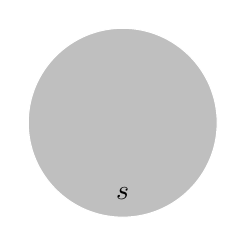
\begin{tikzpicture}
   \filldraw[fill=gray!50, draw=white] (0, 0) circle (1.2);
   \node at (0, -0.9) {$s$};
  \end{tikzpicture}
  \hspace{20pt}
  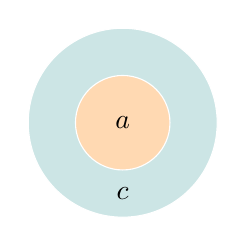
\begin{tikzpicture}
   \filldraw[fill=blue!50!green!20, draw=white] (0, 0) circle (1.2);
   \filldraw[fill=orange!30, draw=white] (0, 0) circle (0.6);
   \node at (0, 0) {$a$};
   \node at (0, -0.9) {$c$};
  \end{tikzpicture}
 \]

 可以从这种存在形式中推导出 \hask{get}/\hask{set} 版本的透镜。
 \begin{haskell}
  toGet :: LensE s a -> (s -> a)
  toGet (LensE (l, r)) = snd . l

  toSet :: LensE s a -> (s -> a -> s)
  toSet (LensE (l, r)) s a = r (fst (l s), a)
 \end{haskell}

 注意,我们不需要知道剩余部分的类型。我们利用了存在透镜包含了 \hask{c} 的生产者和消费者这一事实,而我们只是调解它们之间的关系。

 提取“裸”剩余部分是不可能的,正如以下代码无法编译所证明的那样:
 \begin{haskell}
  getResidue :: Lens s a -> c
  getResidue (Lens (l, r)) = fst . l
 \end{haskell}

 \subsection{范畴论中的存在透镜(Existential Lens in Category Theory)}

 我们可以很容易地将透镜的新定义翻译到范畴论中,使用余极限(coend)表达存在类型:
 \[ \int^{c} \mathcal{C}(s, c \times a) \times  \mathcal{C}(c \times a, s) \]
 事实上,我们可以将其推广为类型变化透镜,其中焦点 $a$ 可以被替换为新类型 $b$ 的焦点。将 $a$ 替换为 $b$ 会产生一个新的复合对象 $t$:
 \[
  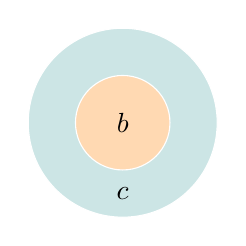
\begin{tikzpicture}
   \filldraw[fill=blue!50!green!20, draw=white] (0, 0) circle (1.2);
   \filldraw[fill=orange!30, draw=white] (0, 0) circle (0.6);
   \node at (0, 0) {$b$};
   \node at (0, -0.9) {$c$};
  \end{tikzpicture}
  \hspace{20pt}
  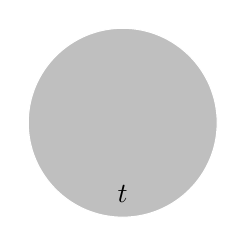
\begin{tikzpicture}
   \filldraw[fill=gray!50, draw=white] (0, 0) circle (1.2);
   \node at (0, -0.9) {$t$};
  \end{tikzpicture}
 \]

 透镜现在由两对对象参数化:$\langle s, t\rangle$ 为外部对象对,$\langle a, b \rangle$ 为内部对象对。存在剩余 $c$ 仍然是隐藏的:
 \[ \mathcal{L}\langle s, t\rangle \langle a, b \rangle = \int^{c} \mathcal{C}(s, c \times a) \times  \mathcal{C}(c \times b, t) \]
 余极限下的乘积是一个在 $y$ 上协变、在 $x$ 上逆变的伴随态射的对角部分:
 \[ \mathcal{C}(s, y \times a) \times  \mathcal{C}(x \times b, t) \]
 \begin{exercise}
  证明:
  \[ \mathcal{C}(s, y \times a) \times  \mathcal{C}(x \times b, t) \]
  是一个在 $\langle x, y\rangle$ 上的伴随态射。
 \end{exercise}

 \subsection{Haskell 中的类型变化透镜(Type-changing Lens in Haskell)}

 在 Haskell 中,我们可以定义一个类型变化透镜为以下存在类型:
 \begin{haskell}
  data LensE s t a b where
  LensE :: (s -> (c, a)) -> ((c, b) -> t) -> LensE s t a b
 \end{haskell}

 和之前一样,我们可以使用存在透镜来获取和设置焦点:
 \begin{haskell}
  toGet :: LensE s t a b -> (s -> a)
  toGet (LensE l r) = snd . l

  toSet :: LensE s t a b -> (s -> b -> t)
  toSet (LensE l r) s a = r (fst (l s), a)
 \end{haskell}

 这两个函数,\hask{s->(c, a)} 和 \hask{(c, b)->t},通常被称为\emph{前向}和\emph{后向}传递。
 前向传递可以用于提取焦点 \hask{a}。后向传递提供了一个问题的答案:如果我们希望前向传递的结果是另一个 \hask{b},我们应该传递给它什么 \hask{t}?

 有时我们只是问:如果我们希望通过 \hask{b} 更改焦点,我们应该对输入进行什么更改 \hask{t}?这种观点在使用透镜描述\index{神经网络}神经网络(neural networks)时特别有用。

 透镜的最简单示例作用于乘积。它可以提取或替换乘积的一个分量,将另一个分量视为剩余部分。在 Haskell 中,我们将其实现为:
 \begin{haskell}
  prodLens :: LensE (c, a) (c, b) a b
  prodLens = LensE id id
 \end{haskell}
 在这里,整体的类型是乘积 \hask{(c, a)}。当我们将 \hask{a} 替换为 \hask{b} 时,我们最终得到目标类型 \hask{(c, b)}。由于源和目标已经是乘积,存在透镜定义中的两个函数只是恒等函数。

 \subsection{透镜组合(Lens Composition)}

 使用透镜的主要优点在于它们可以组合。两个透镜的组合使我们可以放大到某个分量的子分量。

 假设我们从一个透镜开始,它使我们可以访问焦点 \hask{a} 并将其更改为 \hask{b}。这个焦点是整体的一部分,由源 \hask{s} 和目标 \hask{t} 描述。

 我们还有一个内部透镜,它可以访问 \hask{a} 内的焦点 \hask{a'},并将其替换为 \hask{b'},从而为我们提供一个新的 \hask{b}。

 现在我们可以构造一个组合透镜,使我们能够在 \hask{s} 和 \hask{t} 中访问 \hask{a'} 和 \hask{b'}。诀窍是意识到我们可以将两个剩余部分的乘积作为新的剩余部分:
 \[
  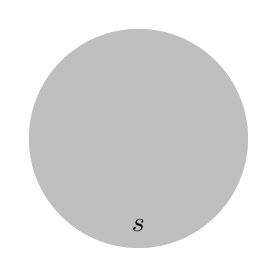
\begin{tikzpicture}
   \filldraw[fill=gray!50, draw=white] (0, 0) circle (1.4);
   \node at (0, -1.1) {$s$};
  \end{tikzpicture}
  \hspace{20pt}
  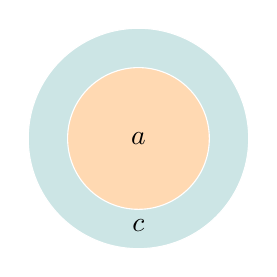
\begin{tikzpicture}
   \filldraw[fill=blue!50!green!20, draw=white] (0, 0) circle (1.4);
   \filldraw[fill=orange!30, draw=white] (0, 0) circle (0.9);
   \node at (0, 0) {$a$};
   \node at (0, -1.1) {$c$};
  \end{tikzpicture}
  \hspace{20pt}
  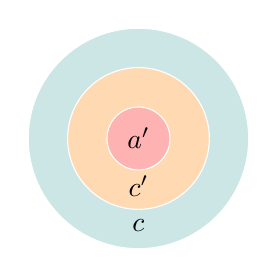
\begin{tikzpicture}
   \filldraw[fill=blue!50!green!20, draw=white] (0, 0) circle (1.4);
   \filldraw[fill=orange!30, draw=white] (0, 0) circle (0.9);
   \filldraw[fill=red!30, draw=white] (0, 0) circle (0.4);
   \node at (0, 0) {$a'$};
   \node at (0, -0.6) {$c'$};
   \node at (0, -1.1) {$c$};
  \end{tikzpicture}
 \]

 \[
  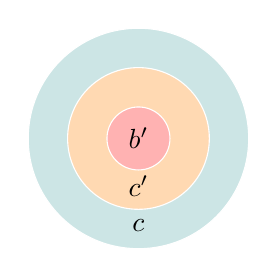
\begin{tikzpicture}
   \filldraw[fill=blue!50!green!20, draw=white] (0, 0) circle (1.4);
   \filldraw[fill=orange!30, draw=white] (0, 0) circle (0.9);
   \filldraw[fill=red!30, draw=white] (0, 0) circle (0.4);
   \node at (0, 0) {$b'$};
   \node at (0, -0.6) {$c'$};
   \node at (0, -1.1) {$c$};
  \end{tikzpicture}
  \hspace{20pt}
  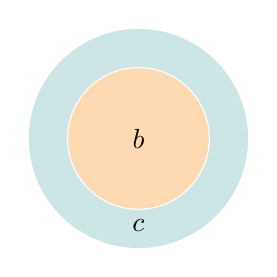
\begin{tikzpicture}
   \filldraw[fill=blue!50!green!20, draw=white] (0, 0) circle (1.4);
   \filldraw[fill=orange!30, draw=white] (0, 0) circle (0.9);
   \node at (0, 0) {$b$};
   \node at (0, -1.1) {$c$};
  \end{tikzpicture}
  \hspace{20pt}
  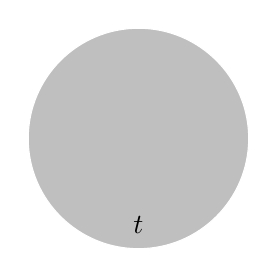
\begin{tikzpicture}
   \filldraw[fill=gray!50, draw=white] (0, 0) circle (1.4);
   \node at (0, -1.1) {$t$};
  \end{tikzpicture}
 \]



 \begin{haskell}
  compLens :: LensE a b a' b' -> LensE s t a b -> LensE s t a' b'
  compLens (LensE l2 r2) (LensE l1 r1) = LensE l3 r3
  where l3 = assoc' . bimap id l2  . l1
  r3 = r1 . bimap id r2 . assoc
 \end{haskell}
 新透镜中的左映射由以下组合给出:
 \[ s \xrightarrow{l_1} (c, a)   \xrightarrow{(id, l_2)} (c, (c', a'))  \xrightarrow{assoc'} ((c, c'), a')\]
 右映射由以下公式给出:
 \[ ((c, c'), b') \xrightarrow{assoc}  (c, (c', b')) \xrightarrow{(id, r_2)} (c, b) \xrightarrow{r_1} t \]

 我们使用了乘积的结合性和函子性:
 \begin{haskell}
  assoc :: ((c, c'), b') -> (c, (c', b'))
  assoc ((c, c'), b') = (c, (c', b'))

  assoc' :: (c, (c', a')) -> ((c, c'), a')
  assoc' (c, (c', a')) = ((c, c'), a')

  instance Bifunctor (,) where
  bimap f g (a, b) = (f a, g b)
 \end{haskell}

 作为示例,让我们组合两个乘积透镜:
 \begin{haskell}
  l3 :: LensE (c, (c', a')) (c, (c', b')) a' b'
  l3 = compLens prodLens prodLens
 \end{haskell}
 并将其应用于嵌套的乘积:
 \begin{haskell}
  x :: (String, (Bool, Int))
  x = ("Outer", (True, 42))
 \end{haskell}
 我们的组合透镜不仅让我们检索最内层的组件:
 \begin{haskell}
  toGet l3 x
  > 42
 \end{haskell}
 还可以用不同类型的值(这里是 \hask{Char})替换它:
 \begin{haskell}
  toSet l3 x 'z'
  > ("Outer",(True,'z'))
 \end{haskell}

 \subsection{透镜的范畴(Category of Lenses)}

 由于透镜可以组合,你可能会想知道是否存在一个范畴,其中透镜作为同态集(hom-sets)。

 确实存在一个范畴 $\mathbf{Lens}$,其对象是 $\mathcal{C}$ 中对象的对,而从 $\langle s, t\rangle$ 到 $ \langle a, b \rangle$ 的箭头是 $\mathcal{L} \langle s, t\rangle \langle a, b \rangle$ 的元素。

 存在透镜的组合公式太复杂,以至于在实际操作中难以使用。在下一章中,我们将看到使用 Tambara 模块表示透镜的另一种表示法,其中组合只是函数的组合。

 \section{透镜与纤维丛 (Lenses and Fibrations)}

 透镜可以通过纤维丛的语言来理解。定义纤维化的投影 $p$ 可以被看作将丛 $E$ 分解为纤维的过程。

 在这种观点下,$p$ 扮演了 \hask{get} 的角色:
 \[ p \colon E \to B \]
 其中 $B$ 代表焦点的类型,而 $E$ 代表可以从中提取出焦点的复合类型。

 透镜的另一部分 \hask{set} 是一个映射:
 \[ q \colon E \times B \to E \]
 让我们看看如何使用纤维化解释它。

 \subsection{传输定律 (Transport Law)}

 我们将 $q$ 解释为将丛 $E$ 的一个元素“传输”到新纤维的操作。新纤维由 $B$ 的一个元素指定。

 传输的这种特性由 get/set 透镜定律,即\emph{传输}定律来表达,它说明“你得到的就是你设置的”:
 \begin{haskell}
  get (set s a) = a
 \end{haskell}
 我们说 $q(s, a)$ 将 $s$ 传输到 $a$ 上的新纤维:

 \[
  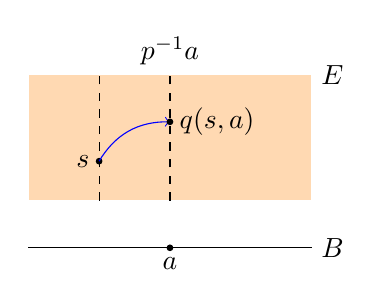
\begin{tikzpicture}

   \def\yb{0}; % base
   \def\yfb{0.6}; % fiber bottom
   \def\yfs{1.1}; % s
   \def\yfss{1.6}; % s'
   \def\yft{2.2}; % fiber top

   \def\dx{0.9};

   \def\xbl{0};
   \def\xbm{\xbl + \dx};
   \def\xbmr{\xbl + 2*\dx};
   \def\xbr{\xbl + 4*\dx};


   \filldraw[fill=orange!30, draw=white] (\xbl, \yfb) rectangle (\xbr, \yft);

   \draw (\xbl, \yb) -- (\xbr, \yb);

   \draw[dashed] (\xbm, \yfb) -- (\xbm, \yft); %fiber
   \draw[dashed] (\xbmr, \yfb) -- (\xbmr, \yft); %fiber

   \filldraw[black] (\xbm, \yfs) circle (1 pt);
   \node[left] at (\xbm, \yfs) {$s$};
   \draw[blue] (\xbm, \yfs) edge[->, bend left] (\xbmr, \yfss);
   \filldraw[black] (\xbmr, \yfss) circle (1 pt);
   \node[right] at (\xbmr, \yfss) {$q(s, a)$};

   \filldraw[black] (\xbmr, \yb) circle (1 pt);
   \node[below] at (\xbmr, \yb) {$a$};

   \node[above] at (\xbmr, \yft) {$p^{-1} a$};
   \node[right] at (\xbr, \yb) {$B$};
   \node[right] at (\xbr, \yft) {$E$};

  \end{tikzpicture}
 \]

 我们可以用 $p$ 和 $q$ 来重新表达这个定律:
 \[ p \circ q = \pi_2 \]
 其中 $\pi_2$ 是从乘积到第二个分量的投影。

 等价地,我们可以将其表示为一个交换图:
 \[
  \begin{tikzcd}
   E \times B
   \arrow[dd, "\varepsilon \times id"']
   \arrow[rd, "q"]
   \\
   & E
   \arrow[dl, "p"]
   \\
   B
  \end{tikzcd}
 \]
 在这里,我使用了一个余单模余单元 $\varepsilon$ 而不是投影 $\pi_2$:
 \[ \varepsilon \colon E \to 1 \]
 然后应用乘积的单位定律。使用余单模使得这个结构更容易推广到单模范畴中的张量积。

 \subsection{恒等定律 (Identity Law)}
 这是 set/get 定律或\emph{恒等}定律。它说明“如果你设置的是你得到的东西,那么不会发生任何变化”:
 \begin{haskell}
  set s (get  s) = s
 \end{haskell}
 我们可以用一个余单模的余乘法来表达:
 \[ \delta \colon E \to E \times E \]
 set/get 定律要求以下组合是一个恒等映射:
 \[ E \xrightarrow{\delta} E \times E \xrightarrow{id \times p} E \times B \xrightarrow{q} E \]
 下图展示了这个定律在丛中的体现:
 \[
  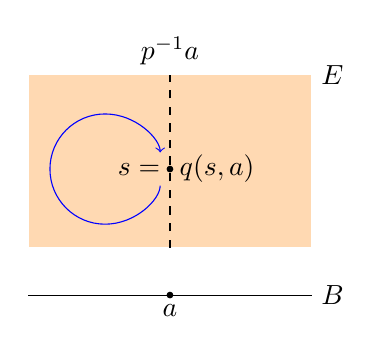
\begin{tikzpicture}

   \def\yb{0}; % base
   \def\yfb{0.6}; % fiber bottom
   \def\yfs{1.1}; % s
   \def\yfss{1.6}; % s'
   \def\yft{2.8}; % fiber top

   \def\dx{0.9};

   \def\xbl{0};
   \def\xbm{\xbl + \dx};
   \def\xbmr{\xbl + 2*\dx};
   \def\xbr{\xbl + 4*\dx};


   \filldraw[fill=orange!30, draw=white] (\xbl, \yfb) rectangle (\xbr, \yft);

   \draw (\xbl, \yb) -- (\xbr, \yb);

   \draw[dashed] (\xbmr, \yfb) -- (\xbmr, \yft); %fiber

   \node at (\xbmr, \yfss) (s) {};
   \draw[->,shorten <=6pt,shorten >=6pt, blue](s.west)arc(360:0:0.7);
   \filldraw[black] (\xbmr, \yfss) circle (1 pt);
   \node[left] at (\xbmr, \yfss) {$s = $};
   \node[right] at (\xbmr, \yfss) {$q(s, a)$};

   \filldraw[black] (\xbmr, \yb) circle (1 pt);
   \node[below] at (\xbmr, \yb) {$a$};

   \node[above] at (\xbmr, \yft) {$p^{-1} a$};
   \node[right] at (\xbr, \yb) {$B$};
   \node[right] at (\xbr, \yft) {$E$};

  \end{tikzpicture}
 \]

 \subsection{组合定律 (Composition Law)}

 最后,这是 set/set 定律或\emph{组合}定律。它说明“最后设置的值获胜”:
 \begin{haskell}
  set (set s a) a' = set s a'
 \end{haskell}
 对应的交换图如下:
 \[
  \begin{tikzcd}
   E \times B \times B
   \arrow[d, "id \times \varepsilon \times id"']
   \arrow[rd, "q \times id"]
   \\
   E \times B
   \arrow[d, "q"']
   & E \times B
   \arrow[dl, "q "]
   \\
   E
  \end{tikzcd}
 \]
 同样地,为了去除中间的 $B$,我使用了余单元而不是从乘积中的投影。

 这就是 set/set 定律在丛中的样子:
 \[
  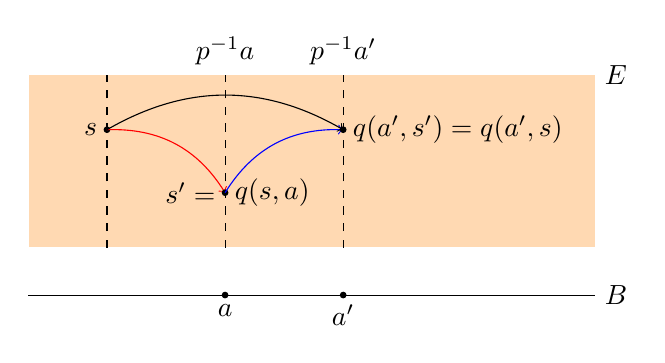
\begin{tikzpicture}

   \def\yb{0}; % base
   \def\yfb{0.6}; % fiber bottom
   \def\yfs{1.3}; % s'
   \def\yfss{2.1}; % s''
   \def\yft{2.8}; % fiber top

   \def\dx{1};

   \def\xbl{0};
   \def\xbm{\xbl + \dx};
   \def\xbmr{\xbl + 2.5*\dx};
   \def\xbmrr{\xbl + 4*\dx};
   \def\xbr{\xbl + 7.2*\dx};


   \filldraw[fill=orange!30, draw=white] (\xbl, \yfb) rectangle (\xbr, \yft);

   \draw (\xbl, \yb) -- (\xbr, \yb);

   \draw[dashed] (\xbm, \yfb) -- (\xbm, \yft); %fiber
   \draw[dashed] (\xbmr, \yfb) -- (\xbmr, \yft); %fiber
   \draw[dashed] (\xbmrr, \yfb) -- (\xbmrr, \yft); %fiber

   \filldraw[black] (\xbm, \yfss) circle (1 pt);
   \node[left] at (\xbm, \yfss) {$s$};

   \draw[red] (\xbm, \yfss)  edge[->, bend left]  (\xbmr, \yfs);

   \filldraw[black] (\xbmr, \yfs) circle (1 pt);
   \node[right] at (\xbmr, \yfs) {$q(s, a)$};
   \node[left] at (\xbmr, \yfs) {$s' =$};

   \draw[blue] (\xbmr, \yfs) edge[->, bend left] (\xbmrr, \yfss);

   \filldraw[black] (\xbmrr, \yfss) circle (1 pt);
   \node[right] at (\xbmrr, \yfss) {$q(a', s') = q(a', s)$};

   \draw (\xbm, \yfss) edge[->, bend left] (\xbmrr, \yfss);


   \filldraw[black] (\xbmr, \yb) circle (1 pt);
   \node[below] at (\xbmr, \yb) {$a$};

   \filldraw[black] (\xbmrr, \yb) circle (1 pt);
   \node[below] at (\xbmrr, \yb) {$a'$};

   \node[above] at (\xbmr, \yft) {$p^{-1} a$};
   \node[above] at (\xbmrr, \yft) {$p^{-1} a'$};
   \node[right] at (\xbr, \yb) {$B$};
   \node[right] at (\xbr, \yft) {$E$};

  \end{tikzpicture}
 \]

 \subsection{类型转换透镜 (Type-changing Lens)}

 类型转换透镜将传输泛化为在丛之间操作。我们必须定义一整个丛的家族。我们从一个范畴 $\cat A$ 开始,其对象定义了我们将用于透镜焦点的类型。

 我们构造集合 $B$ 作为所有焦点类型的所有元素的联合集合。$B$ 在 $\cat A$ 上纤维化——投影 $\pi$ 将 $B$ 的一个元素发送到其对应的类型。你可以将 $B$ 视为余切范畴 $1/ \cat A$ 的对象集合。

 丛的丛 $E$ 是一个在 $B$ 上纤维化的集合,其投影为 $p$。由于 $B$ 本身在 $\cat A$ 上纤维化,$E$ 在 $\cat A$ 上传递地纤维化,投影为复合投影 $\pi \circ p$。正是这种更粗的纤维化将 $E$ 分解为一个丛的家族。每个丛对应于给定焦点类型的复合类型的不同类型。类型转换透镜将在这些丛之间移动。

 \[
  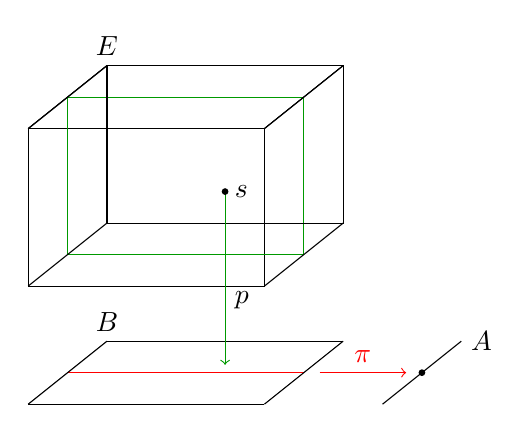
\begin{tikzpicture}
   \def\xl{-3};
   \def\xr{0};
   \def\yb{0};
   \def\yt{2};

   \def\dy{0.4};
   \def\dx{0.5};

   \def\a{(\xl, \yb)};
   \def\b{(\xr, \yb)};
   \def\c{(\xl, \yt)};
   \def\d {(\xr, \yt)};

% _a second plane
   \def\aa{(\xl + \dx, \yb + \dy)};
   \def\ba{(\xr + \dx, \yb + \dy)};
   \def\ca{(\xl + \dx, \yt + \dy)};
   \def\da{(\xr + \dx, \yt + \dy)};

% _b third plane
   \def\ab{(\xl + 2*\dx, \yb + 2*\dy)};
   \def\bb{(\xr + 2*\dx, \yb + 2*\dy)};
   \def\cb{(\xl + 2*\dx, \yt + 2*\dy)};
   \def\db{(\xr + 2*\dx, \yt + 2*\dy)};

% shifted walls
   \def\yshift{-1.5};
   \def\xshift{1.5};

% E
   \draw \a rectangle \d;
   \draw[draw=black!40!green] \aa rectangle \da;
   \draw \ab rectangle \db;

   \draw \a -- \ab;
   \draw \b -- \bb;
   \draw \d -- \db;
   \draw \c -- \cb;

   \node[above] at \cb {$E$};

% B
% rebase yb (bottom)
   \def\yb{\yshift}
% rebase xr (right wall)
   \def\xr{0};

   \draw \a -- \b;
   \draw \ab -- \bb;
   \draw[red] \aa -- \ba;
% diagonal
   \draw \a -- \ab;
   \draw \b -- \bb;
   \draw \d -- \db;
   \draw \c -- \cb;
   \node[above] at \ab {$B$};


% A
% rebase yb (bottom)
   \def\yb{\yshift}
% rebase xr (right wall)
   \def\xr{\xshift};

   \draw \b -- \bb;
   \node[right] at \bb {$\cat A$};
   \filldraw[black] \ba circle (1 pt);

%projections

   \draw[red, shorten <=0.2cm, shorten >=0.2cm, ->] (0 + \dx, \yshift + \dy) -- node[above]{$\pi$} (\xshift +\dx, \yshift + \dy);

   \draw[draw=black!40!green, shorten >=0.1cm, ->] (0 - \dx, 0 + 3 * \dy) -- node[below right]{$p$} (0 - \dx, \yshift + \dy);

   \node[right] at (0 - \dx, 0 + 3 * \dy) {$s$};
   \filldraw[black] (0 - \dx, 0 + 3 * \dy) circle (1 pt);


  \end{tikzpicture}
 \]

 投影 $p$ 将元素 $s \in E$ 转换为一个元素 $b \in B$,其类型由 $\pi b$ 给出。这是 \hask{get} 的推广。

 对应于 \hask{set} 的传输 $q$ 接收一个元素 $s \in E$ 和一个元素 $b \in B$,并生成一个新元素 $t \in E$。重要的是要注意,$s$ 和 $t$ 可以属于 $E$ 的不同子丛。

 传输满足以下定律:

 get/set 定律(传输):

 \[ p (q (b, s)) = b \]

 set/get 定律(恒等):

 \[ q ( p (s), s) = s \]

 set/set 定律(组合):

 \[ q (c, q (b, s)) = q (c, s) \]

 \section{重要公式 (Important Formulas)}
 这是一个便捷的(共)端计算速查表。
 \begin{itemize}
  \item Hom-函子连续性 (Continuity of the hom-functor):
  \[\cat D\left(d, \int_a P\langle a, a \rangle \right) \cong \int_a \cat D \left(d, P\langle a, a \rangle \right) \]
  \item Hom-函子共连续性 (Co-continuity of the hom-functor):
  \[\cat D\left( \int^a P\langle a, a \rangle , d \right) \cong \int_a \cat D \left( P\langle a, a \rangle, d \right) \]
  \item 忍者 Yoneda (Ninja Yoneda):
  \[ \int_{x} \mathbf{Set} (\mathcal{C}(a, x), F x) \cong F a \]
  \item 忍者 Co-Yoneda (Ninja co-Yoneda):
  \[ \int^{x} \mathcal{C}(x, a) \times F x \cong F a \]
  \item 反变函子(预层)的忍者 Yoneda (Ninja Yoneda for contravariant functors):
  \[ \int_{x} \mathbf{Set} (\mathcal{C}(x, a), G x) \cong G a \]
  \item 反变函子(预层)的忍者 Co-Yoneda (Ninja co-Yoneda for contravariant functors):
  \[ \int^{x} \mathcal{C}(a, x) \times G x \cong G a \]
  \item Day 卷积 (Day Convolution):
  \[ (F \star G) x = \int^{a, b} \cat C (a \otimes b, x) \times F a \times G b \]

 \end{itemize}


\end{document}